
\chapter{UML-Diagramme}

\paragraph{} Die UML-Diagramme wurden mit der Software UMLet erstellt (siehe: \url{http://www.umlet.com/}, Stand 29.08.2012 bzw. M. Auer, T. Tschurtschenthaler, S. Biffl: A Flyweight UML Modelling Tool for Software Development in Heterogeneous Environments, Proceeding EUROMICRO '03; Proceedings of the 29th Conference on EUROMICRO, S. 267).

\section{Domänenmodell}
\label{uml-domain}

\begin{textblock}{3}(0.5,8)
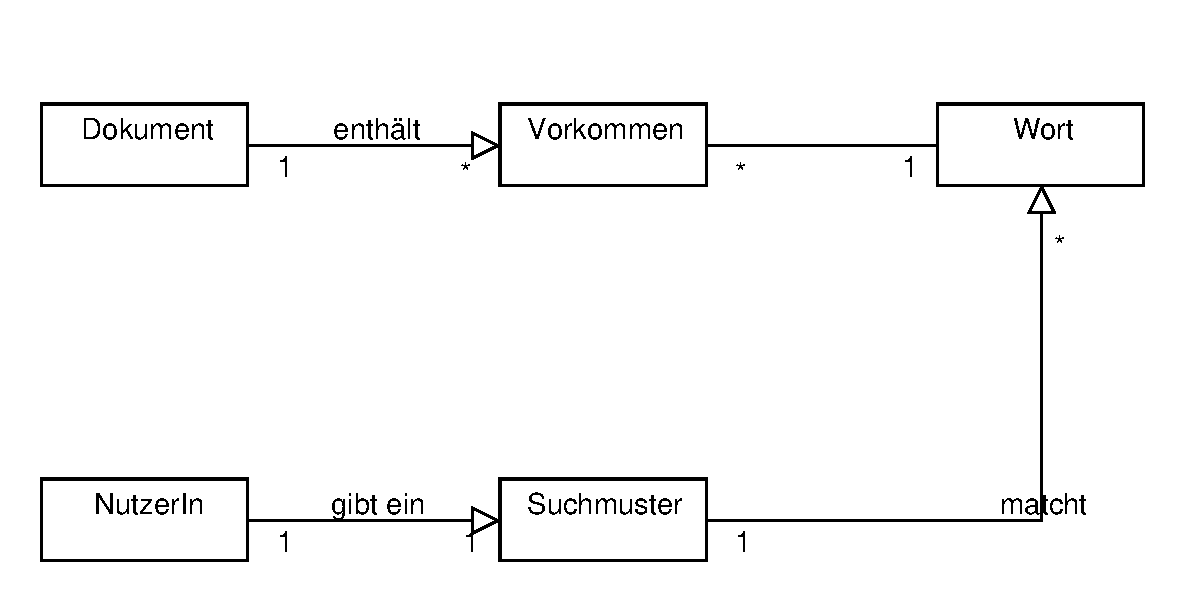
\includegraphics[scale=1]{resources/domain-model.pdf}
\end{textblock}
\newpage

\section{Architekturkonzept}
\label{uml-architecture}

\begin{textblock}{3}(3,3)
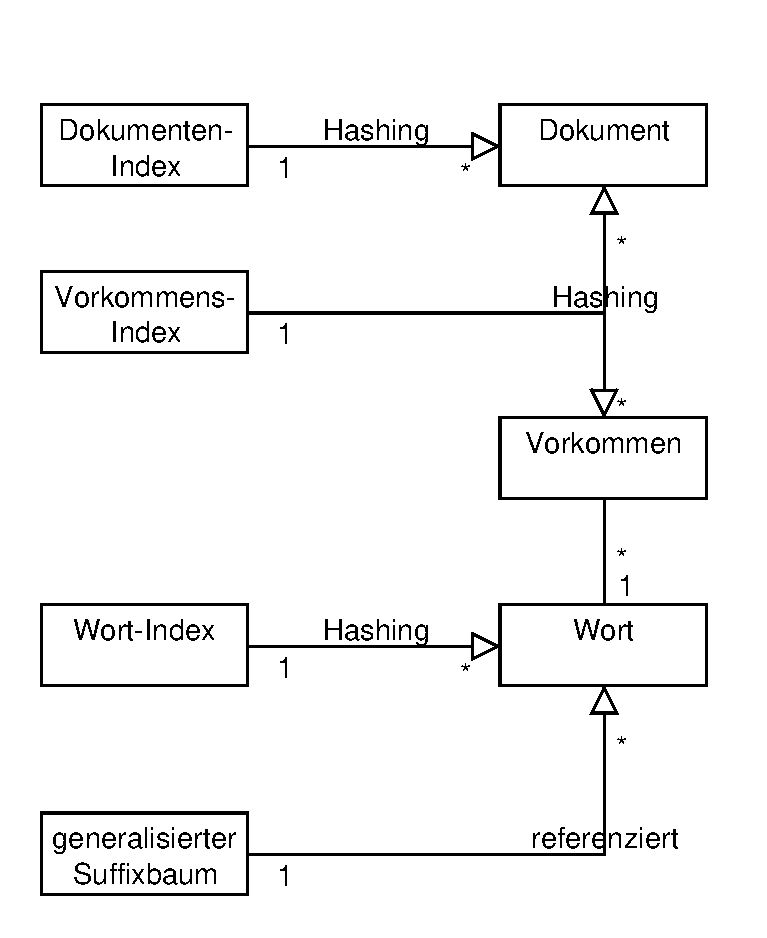
\includegraphics[scale=1]{resources/architecture.pdf}
\end{textblock}
\newpage

\section{Paketdiagramm}
\label{uml-package}

\begin{textblock}{3}(0.5,4)
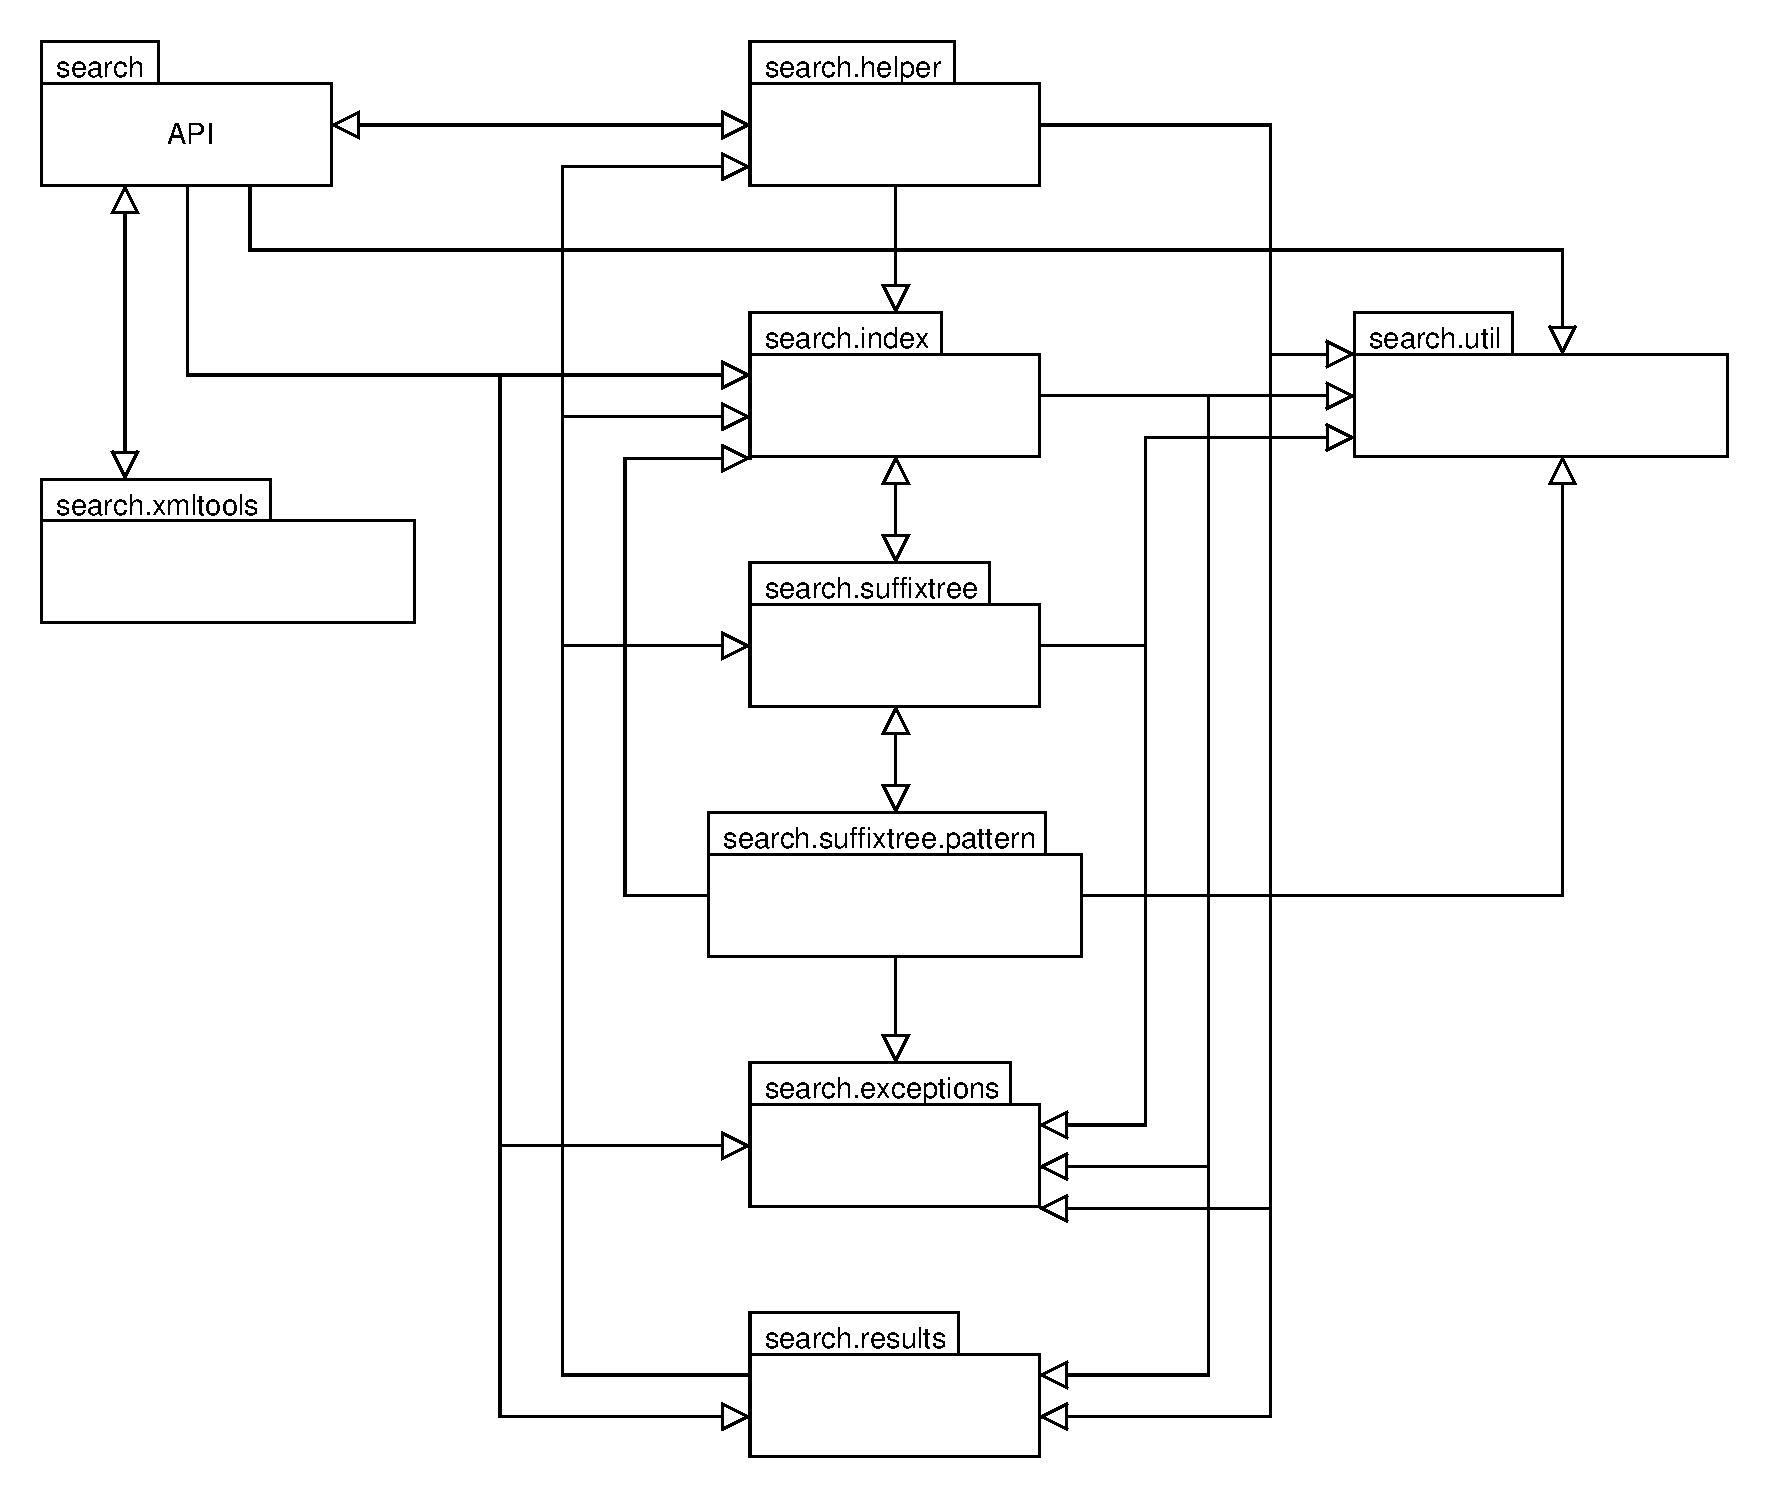
\includegraphics[scale=0.68]{resources/packages.pdf}
\end{textblock}

\newpage

\section{Klassendiagramm}
\label{uml-classes}

\begin{textblock}{3}(0.5,2.5)
\includegraphics[angle=270,scale=0.5]{resources/classes.pdf}
\end{textblock}

\newpage